\section*{Chương 1: Cơ sở lý thuyết về biến đổi Haar Wavelet}
\addcontentsline{toc}{section}{Chương 1: Cơ sở lý thuyết về biến đổi Haar Wavelet}

\subsection*{1. Tổng quan về phép biến đổi Wavelet và Haar Wavelet}
Wavelet trong tiếng Pháp còn được hiểu là sóng con. Trong toán học, Wavelet đại diện cho những hàm sóng
có thể được co dãn và tịnh tiến. Một biến đổi Wavelet có thể biến bất kỳ tín hiệu nào thành các tín hiệu được xây dựng
từ các sóng con này.

Alfred Haar (1885-1933) là nhà toán học người Hungary, người đã giới thiệu biến đổi Haar Wavelet vào năm 1909. 
Đây là loại Wavelet đơn giản nhất, không có sự chồng chéo, chia tín hiệu thành các cặp giá trị rời rạc và xử lý cục bộ.

Biến đổi Haar Wavelet hoạt động bằng cách phân tách tín hiệu rời rạc thành hai phần có độ dài bằng nhau: 
thành phần trung bình (average) giữ lại cấu trúc tổng thể và thành phần sai khác (difference) lưu giữ những chi tiết sắc nét.
Đặc biệt hơn từ hai thành phần này ta có thể khôi phục lại được tín hiệu ban đầu một cách vô cùng chính xác. 

\subsection*{2. Phép biến đổi Haar 1D}
Để xem việc phân tích một tín hiệu bằng cách tính trung bình và sai khác như thế nào ta có thể xét một đoạn tín hiệu như sau:
$$X_{0}=(154, 150, 156, 152, 160, 160, 152, 156)^T$$
Ta chia đoạn tín hiệu trên thành từng cặp và tìm nửa tổng, nửa hiệu của các cặp đó. Ta sẽ thu được một dãy sau:
$$X_{1}=(152, 154, 160, 154, 2, 2, 0, -2)$$
Trong dãy $X_{1}$ trên, bốn số đầu tiên là nửa tổng của bốn cặp, bốn số tiếp theo là nửa hiệu của bốn cặp.
Ta có thể dùng ma trận để mô tả quá trình này như sau:
\begin{center}
    $$A = \begin{pmatrix}
        \frac{1}{2} &  \frac{1}{2} &  0 &  0 &  0 &  0 &  0 &  0 \\
        0 &  0 &  \frac{1}{2} &  \frac{1}{2} &  0 &  0 &  0 &  0 \\
        0 &  0 &  0 &  0 &  \frac{1}{2} &  \frac{1}{2} &  0 &  0 \\
        0 &  0 &  0 &  0 &  0 &  0 &  \frac{1}{2} &  \frac{1}{2} \\
        \frac{1}{2} & -\frac{1}{2} &  0 &  0 &  0 &  0 &  0 &  0 \\
        0 &  0 &  \frac{1}{2} & -\frac{1}{2} &  0 &  0 &  0 &  0 \\
        0 &  0 &  0 &  0 &  \frac{1}{2} & -\frac{1}{2} &  0 &  0 \\
        0 &  0 &  0 &  0 &  0 &  0 &  \frac{1}{2} & -\frac{1}{2}
    \end{pmatrix}$$
\end{center}

Ta thấy rằng nếu lấy tích vô hướng của từng hàng với nhau kết quả đều là 0, điều này cho thấy các hàng của ma trận $A$ tạo nên họ trực giao.
Nếu ta chia mỗi hàng cho độ dài của chúng ta được họ trực chuẩn, ma trận trực giao $H$ tương ứng như sau:
\begin{center}
    $$H = \begin{pmatrix}
        \frac{\sqrt{2}}{2} &  \frac{\sqrt{2}}{2} &  0 &  0 &  0 &  0 &  0 &  0 \\
        0 &  0 &  \frac{\sqrt{2}}{2} &  \frac{\sqrt{2}}{2} &  0 &  0 &  0 &  0 \\
        0 &  0 &  0 &  0 &  \frac{\sqrt{2}}{2} &  \frac{\sqrt{2}}{2} &  0 &  0 \\
        0 &  0 &  0 &  0 &  0 &  0 &  \frac{\sqrt{2}}{2} &  \frac{\sqrt{2}}{2} \\
        \frac{\sqrt{2}}{2} & -\frac{\sqrt{2}}{2} &  0 &  0 &  0 &  0 &  0 &  0 \\
        0 &  0 &  \frac{\sqrt{2}}{2} & -\frac{\sqrt{2}}{2} &  0 &  0 &  0 &  0 \\
        0 &  0 &  0 &  0 &  \frac{\sqrt{2}}{2} & -\frac{\sqrt{2}}{2} &  0 &  0 \\
        0 &  0 &  0 &  0 &  0 &  0 &  \frac{\sqrt{2}}{2} & -\frac{\sqrt{2}}{2}
    \end{pmatrix}$$
\end{center}

Khi đã xây dựng được ma trận $H$, vì $H$ là ma trận trực giao nên nghịch đảo của $H$ là $H^T$. 
Ta dùng ma trận $H$ để nén dữ liệu thay vì dùng ma trận $A$. Nén dữ liệu $X_{0}$ ta được $Y_{1}=HX_{0}$.
Giải nén dữ liệu từ $Y_{1}$ ta được $X_{0}=H^TY_{1}$.
Phép biến đổi tín hiệu dùng ma trận trực giao $H$ là vô cùng quan trọng vì nó có nhiều tính chất như sau:

Tính bảo toàn độ dài vector. Cho $X$ là một vector, ta có
$$||HX||=\sqrt{(HX)^T(HX)}=\sqrt{X^TH^THX}=\sqrt{X^TX}=||X||$$

Tính bảo toàn tích vô hướng. Cho $u$ và $v$ là hai vector, ta có
$$(Hu,Hv)=(Hu)^T.(Hv)=u^TH^THv=u^Tv=(u,v)$$

Tính bảo toàn góc giữa hai vector. Cho hai vector $u$ và $v$ thỏa $cos\theta=\frac{(u,v)}{||u||.||v||}$, ta có
$$cos\psi=\frac{(Hu,Hv)}{||Hu||.||Hv||}=\frac{(u,v)}{||u||.||v||}=cos\theta$$

Phép biến đổi bằng ma trận trực giao $H$ bảo toàn góc và khoảng cách giữa các vector nên  nó không làm thay đổi hình dạng của ảnh trong quá trình nén.

Tiếp tục quá trình nén ở trên, cho ma trận $H_{1}$ là ma trận $H$ đã phân tích, khi đó $Y_{1}=H_{1}X_{0}=\sqrt{2}(152, 154, 160, 154, 2, 2, 0, -2)^T$.
Quá trình nén tiếp theo ta giữ lại bốn số sau của dãy và thực hiện lấy nửa tổng và nửa hiệu của các cặp số trong bốn số đầu ta được 
$Y_{2}=H_{2}Y_{1}=(306,314,-2,6,2\sqrt{2},2\sqrt{2},0,-2\sqrt{2})^T$. Ma trận $H_{2}$ được mô tả như sau
\begin{center}
    $$H_2 = \begin{pmatrix}
        \frac{\sqrt{2}}{2} &  \frac{\sqrt{2}}{2} &  0 &  0 &  0 &  0 &  0 &  0 \\
        0 &  0 &  \frac{\sqrt{2}}{2} &  \frac{\sqrt{2}}{2} &  0 &  0 &  0 &  0 \\
        \frac{\sqrt{2}}{2} & -\frac{\sqrt{2}}{2} &  0 &  0 &  0 &  0 &  0 &  0 \\
        0 &  0 &  \frac{\sqrt{2}}{2} & -\frac{\sqrt{2}}{2} &  0 &  0 &  0 &  0 \\
        0 &  0 &  0 &  0 &  1 &  0 &  0 &  0 \\
        0 &  0 &  0 &  0 &  0 &  1 &  0 &  0 \\
        0 &  0 &  0 &  0 &  0 &  0 &  1 &  0 \\
        0 &  0 &  0 &  0 &  0 &  0 &  0 &  1
    \end{pmatrix}$$
\end{center}

Tiếp tục quá trình trên, giữ sáu số cuối của $Y_{2}$ lại và hai số đầu được thay bằng nửa tổng và nửa hiệu của chúng ta được
$Y_{3}=H_{3}Y_{2}=(310\sqrt{2},-4\sqrt{2},-2,6,2\sqrt{2},2\sqrt{2},0,-2\sqrt{2})^T$ với ma trận $H_{3}$ được mô tả như sau
\begin{center}
    $$H_3 = \begin{pmatrix}
        \frac{\sqrt{2}}{2} &  \frac{\sqrt{2}}{2} &  0 &  0 &  0 &  0 &  0 &  0 \\
        \frac{\sqrt{2}}{2} & -\frac{\sqrt{2}}{2} &  0 &  0 &  0 &  0 &  0 &  0 \\
        0 &  0 &  1 &  0 &  0 &  0 &  0 &  0 \\
        0 &  0 &  0 &  1 &  0 &  0 &  0 &  0 \\
        0 &  0 &  0 &  0 &  1 &  0 &  0 &  0 \\
        0 &  0 &  0 &  0 &  0 &  1 &  0 &  0 \\
        0 &  0 &  0 &  0 &  0 &  0 &  1 &  0 \\
        0 &  0 &  0 &  0 &  0 &  0 &  0 &  1
    \end{pmatrix}$$
\end{center}

Nhìn chung ta có được $Y_3=H_3H_2H_1X_0 \iff Y_3=QX_0$. Vector $Y_3$ có phần tử đầu tiên là trung bình tổng thể mang giá trị xấp xỉ cho
cả dãy số ban đầu. Bảy phần tử còn lại là các hệ số chi tiết từ vĩ mô đến vi mô nhất của dãy số, cho biết sự thay đổi từ lớn đến nhỏ của các phần tử ở từng độ phân giải của dãy số.

Ta còn có thể giải nén dữ liệu $Y_3$ để tìm lại dãy ban đầu bằng cách $X_0=Q^{-1}Y_3 \iff X_0=Q^TY_3$ với 

\begin{center}
    $$Q = \begin{pmatrix}
        \frac{\sqrt{2}}{4} &  \frac{\sqrt{2}}{4} &  \frac{\sqrt{2}}{4} &  \frac{\sqrt{2}}{4} &  \frac{\sqrt{2}}{4} &  \frac{\sqrt{2}}{4} &  \frac{\sqrt{2}}{4} &  \frac{\sqrt{2}}{4} \\
        \frac{\sqrt{2}}{4} &  \frac{\sqrt{2}}{4} &  \frac{\sqrt{2}}{4} &  \frac{\sqrt{2}}{4} & -\frac{\sqrt{2}}{4} & -\frac{\sqrt{2}}{4} & -\frac{\sqrt{2}}{4} & -\frac{\sqrt{2}}{4} \\
        \frac{1}{2} &  \frac{1}{2} & -\frac{1}{2} & -\frac{1}{2} &  0 &  0 &  0 &  0 \\
        0 &  0 &  0 &  0 &  \frac{1}{2} &  \frac{1}{2} & -\frac{1}{2} & -\frac{1}{2} \\
        \frac{\sqrt{2}}{2} & -\frac{\sqrt{2}}{2} &  0 &  0 &  0 &  0 &  0 &  0 \\
        0 &  0 &  \frac{\sqrt{2}}{2} & -\frac{\sqrt{2}}{2} &  0 &  0 &  0 &  0 \\
        0 &  0 &  0 &  0 &  \frac{\sqrt{2}}{2} & -\frac{\sqrt{2}}{2} &  0 &  0 \\
        0 &  0 &  0 &  0 &  0 &  0 &  \frac{\sqrt{2}}{2} & -\frac{\sqrt{2}}{2}
    \end{pmatrix}$$
\end{center}
\subsection*{3. Xây dựng ma trận phép biến đổi Haar}

Một ma trận phép biến đổi Haar cuối cùng có thể được tạo thành bằng việc nhân nhiều ma trận với nhau ($Q=H_3H_2H_1$).
Đối với một vector có $2^m$ phần tử ta rốt cuộc phải tìm ra $m$ ma trận trước khi tìm được ma trận cuối cùng. Việc này có thể tốn nhiều thời gian và công sức.
Vì vậy, còn một cách khác để tạo ra ma trận Haar trực giao
đó chính là sử dụng những hàm Haar $h_k(x)$. Những hàm này được định nghĩa với $x \in [0,1]$, $k=0,1,2...,N-1$ và $N=2^n$ (N là lũy thừa cơ số 2).
$$h_0(x)=h_{00}(x)=\frac{1}{\sqrt{N}}, x \in [0,1]$$
và 
$$h_k(x) = h_{pq}(x) = \frac{1}{\sqrt{N}}
\begin{cases} 
    2^{\frac{p}{2}}, & \frac{q-1}{2^p} \leq x < \frac{q-\frac{1}{2}}{2^p} \\[2ex]
    -2^{\frac{p}{2}}, & \frac{q-\frac{1}{2}}{2^p} \leq x < \frac{q}{2^p} \\[2ex]
    0, & \text{các trường hợp khác của } x \in [0, 1]
\end{cases}$$

\noindent Bất kì số nguyên $k$ nào cũng có thể được biểu diễn bằng tổng $k=2^p+q-1$ với $0 \le p \le n-1$. Với $p=0$ thì $q=0$ hoặc $q=1$.
Với $p \ne 0$ thì $1 \le q \le 2^p$.

Ma trận Haar $H_N$ vuông cấp $N \times N$ có thể được xây dựng theo cách: mỗi phần tử $i$ và $j$ là một cơ sở hàm Haar $h_i(j)$ với $i=0,1,2,...,N-1$
và $j=\frac{0}{N},\frac{1}{N},...,\frac{(N-1)}N{}$. Xét một ví dụ ma trận Haar cấp 4 như sau:
\begin{center}
    $$H_4 = \begin{pmatrix}
        h_0(0/4) & h_0(1/4) & h_0(2/4) & h_0(3/4) \\
        h_1(0/4) & h_1(1/4) & h_1(2/4) & h_1(3/4) \\
        h_2(0/4) & h_2(1/4) & h_2(2/4) & h_2(3/4) \\
        h_3(0/4) & h_3(1/4) & h_3(2/4) & h_3(3/4)
    \end{pmatrix} = 
    \frac{1}{\sqrt{4}} \begin{pmatrix}
        1 & 1 & 1 & 1 \\
        1 & 1 & -1 & -1 \\
        \sqrt{2} & -\sqrt{2} & 0 & 0 \\
        0 & 0 & \sqrt{2} & -\sqrt{2}
    \end{pmatrix}$$
\end{center}

\subsection*{4. Phép biến đổi Haar 2D}
Một bức ảnh $2^m \times 2^n$ pixels còn có thể được biểu diễn bởi một ma trận $m \times n$. Nếu bức ảnh là ảnh đơn sắc thì từng phần tử trong ma trận ảnh
biểu diễn độ sáng từ đen đến xám rồi đến trắng của pixel tương ứng. Việc dùng phép biến đổi Haar để nén một bức ảnh có thể được hiểu theo cách 
biến đổi Haar cho từng hàng của bức ảnh sau đó biến đổi Haar cho từng cột của bức ảnh. Xét ví dụ một ma trận ảnh $A_{m \times n}$ có thể được nén thành $B_{m \times n}$ như sau:
$$B_{m \times n} = H_mA_{m \times n}H_n^T$$

\noindent Và được giải nén: $$A_{m \times n} = H_m^{-1}B_{m \times n}(H_n^T)^{-1}$$

Quá trình nén ảnh trên có sự tương đồng với cách hiểu lấy nửa tổng và nửa hiệu cho từng cặp giá trị như biến đổi cho một dãy số. 
Vì việc lấy nửa tổng và nửa hiệu diễn ra trên cả hàng và cả cột, ta có cách hiểu sau về phép biến đổi Haar cho ma trận ảnh. 

Chia ma trận ảnh thành nhiều khối vuông 4 pixel, xét một khối vuông như sau:
\begin{figure}[H]
    \centering
    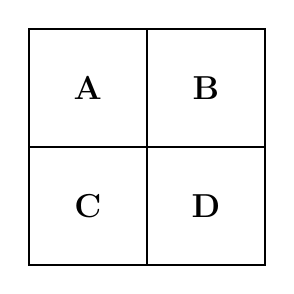
\begin{tikzpicture}[scale=1.5] % Thay đổi scale để phóng to/thu nhỏ toàn bộ hình
        % Vẽ khung hình vuông lớn bên ngoài
        \draw[thick] (0,0) rectangle (2,2);
        
        % Vẽ đường chia ngang và dọc ở giữa
        \draw[thick] (1,0) -- (1,2);
        \draw[thick] (0,1) -- (2,1);
        
        % Đặt các nhãn LL, HL, LH, HH vào giữa các ô
        \node at (0.5, 1.5) {\large \textbf{A}};
        \node at (1.5, 1.5) {\large \textbf{B}};
        \node at (0.5, 0.5) {\large \textbf{C}};
        \node at (1.5, 0.5) {\large \textbf{D}};
    \end{tikzpicture}
    \vspace{0.3cm}
\end{figure}
Sau phép biến đổi Haar một lần cho hàng và cột ta thu được 4 pixel riêng rẽ mới:
\begin{figure}[H]
    \centering
    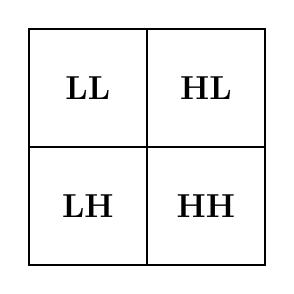
\begin{tikzpicture}[scale=1.5] % Thay đổi scale để phóng to/thu nhỏ toàn bộ hình
        % Vẽ khung hình vuông lớn bên ngoài
        \draw[thick] (0,0) rectangle (2,2);
        
        % Vẽ đường chia ngang và dọc ở giữa
        \draw[thick] (1,0) -- (1,2);
        \draw[thick] (0,1) -- (2,1);
        
        % Đặt các nhãn LL, HL, LH, HH vào giữa các ô
        \node at (0.5, 1.5) {\large \textbf{LL}};
        \node at (1.5, 1.5) {\large \textbf{HL}};
        \node at (0.5, 0.5) {\large \textbf{LH}};
        \node at (1.5, 0.5) {\large \textbf{HH}};
    \end{tikzpicture}
    \vspace{0.3cm}
\end{figure}
Trong đó:
$$LL = \frac{1}{\sqrt{2}} \left[ \frac{1}{\sqrt{2}}(A+B)+\frac{1}{\sqrt{2}}(C+D) \right] =\frac{1}{2}(A+B+C+D)$$
$$HL = \frac{1}{\sqrt{2}} \left[ \frac{1}{\sqrt{2}}(A-B) + \frac{1}{\sqrt{2}}(C-D) \right] = \frac{1}{2}(A-B+C-D)$$
$$LH = \frac{1}{\sqrt{2}} \left[ \frac{1}{\sqrt{2}}(A+B) - \frac{1}{\sqrt{2}}(C+D) \right] = \frac{1}{2}(A+B-C-D)$$
$$HH = \frac{1}{\sqrt{2}} \left[ \frac{1}{\sqrt{2}}(A-B) - \frac{1}{\sqrt{2}}(C-D) \right] = \frac{1}{2}(A-B-C+D)$$

Tập hợp các pixel LL cho ta một bức ảnh đại diện cho thành phần xấp xỉ của bức ảnh ban đầu. 
Tập hợp các pixel HL ta sẽ thu được một ảnh sự khác biệt về chi tiết biên. Tương tự cho các pixel LH và HH. 

\begin{figure}[H]
    \centering
    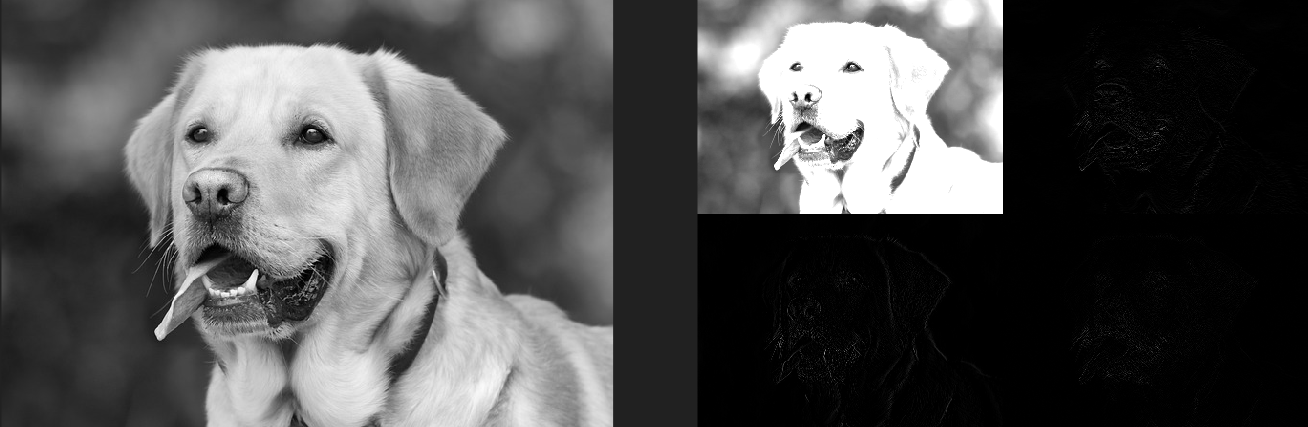
\includegraphics[width=1\textwidth]{Lv1.png}
    \caption{Hình ảnh minh họa phép biến đổi lần 1.}
\end{figure}

\noindent Biến đổi lần 2 đối với ảnh gốc là ảnh LL ta phân tích được nhiều chi tiết hơn

\begin{figure}[H]
    \centering
    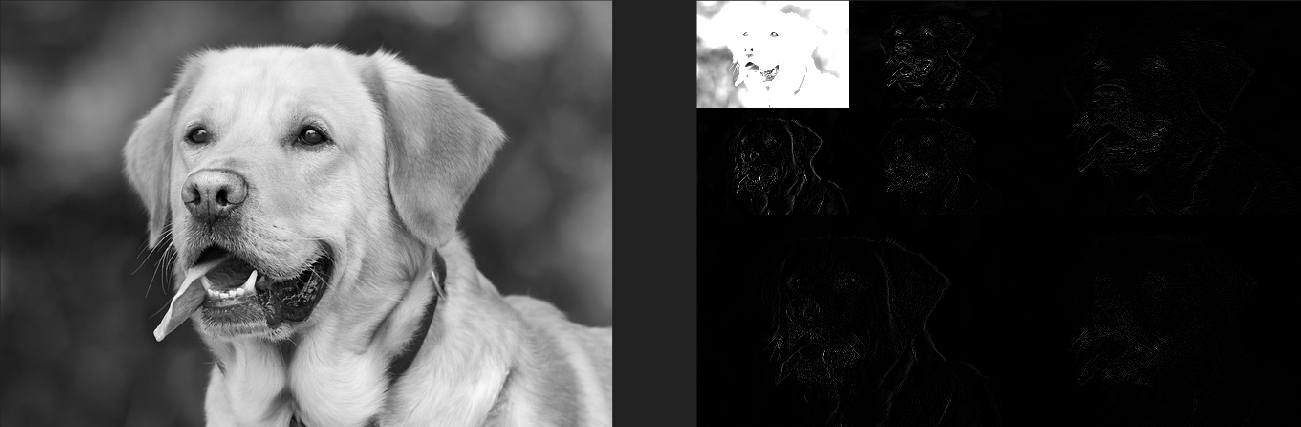
\includegraphics[width=1\textwidth]{Lv2.png}
    \caption{Hình ảnh minh họa phép biến đổi lần 2.}
\end{figure}

\subsection*{Nén không mất dữ liệu và nén mất dữ liệu}
Ý nghĩa thật sự của việc nén ảnh còn nằm ở việc tối đa hóa dữ liệu mà không làm giảm quá nhiều chất lượng ảnh.
Phương pháp này được gọi là nén mất dữ liệu. 

Một ma trận với tỷ lệ nhiều các phần tử bằng 0 được xem là thưa thớt. Đối với các ma trận ảnh, 
ma trận đã biến đổi bằng Haar Wavelet thưa hơn rất nhiều so với ma trận gốc. Hơn hết, các ma trận thưa
đơn giản hóa việc lưu trữ và truyền tải hơn ma trận ảnh gốc.

Điểm đặc biệt nhất của việc nén  mất dữ liệu này là ta có thể điều chỉnh các chi tiết ở 
vùng chi tiết cao để tạo ra nhiều phần tử 0 hơn. Để làm được điều này ta sẽ chọn một giá trị
ngưỡng $\epsilon$ và đưa tất cả hệ số chi tiết nào nhỏ hơn $\epsilon$ về 0. Sau đó ta 
thực hiện giải nén và thu được ảnh gần với ảnh gốc. Thú vị là bức ảnh thu được sau ép ngưỡng và giải 
nén gần như giống hệt ảnh gốc và hầu như rất khó nhận ra khác biệt bằng mắt thường. Phương pháp này 
được gọi là \textit{"Nén không mất dữ liệu"} nếu $\epsilon = 0$, ngược lại được gọi là 
\textit{"Nén mất dữ liệu"} nếu $\epsilon > 0$. 

Lấy ví dụ một ma trận ảnh $P$ như sau:
$$P = \begin{pmatrix}
    576 & 704 & 1152 & 1280 & 1344 & 1472 & 1536 & 1536 \\
    704 & 640 & 1156 & 1088 & 1344 & 1408 & 1536 & 1600 \\
    768 & 832 & 1216 & 1472 & 1472 & 1536 & 1600 & 1600 \\
    832 & 832 &  960 & 1344 & 1536 & 1536 & 1600 & 1536 \\
    832 & 832 &  960 & 1216 & 1536 & 1600 & 1536 & 1536 \\
    960 & 896 &  896 & 1088 & 1600 & 1600 & 1600 & 1536 \\
    768 & 768 &  832 &  832 & 1280 & 1472 & 1600 & 1600 \\
    448 & 768 &  704 &  640 & 1280 & 1408 & 1600 & 1600
\end{pmatrix}.$$
Sau phép biến đổi Haar ta thu được ma trận $T$:
$$T = \begin{pmatrix}
    1212 & -306 & -146 &  -54 &  -24 &  -68 &  -40 &   4 \\
      30 &   36 &  -90 &   -2 &    8 &  -20 &    8 &  -4 \\
     -50 &  -10 &  -20 &  -24 &    0 &   72 &  -16 & -16 \\
      82 &   38 &  -24 &   68 &   48 &  -64 &   32 &   8 \\
       8 &    8 &  -32 &   16 &  -48 &  -48 &  -16 &  16 \\
      20 &   20 &  -56 &  -16 &  -16 &   32 &  -16 & -16 \\
      -8 &    8 &  -48 &    0 &  -16 &  -16 &  -16 & -16 \\
      44 &   36 &    0 &    8 &   80 &  -16 &  -16 &   0
\end{pmatrix}.$$
Lấy ngưỡng $\epsilon = 20$, đưa tất cả hệ số chi tiết có giá trị tuyệt đối nhỏ hơn 20 về 0 ta được ma trận $D$:
$$D = \begin{pmatrix}
    1212 & -306 & -146 &  -54 &  -24 &  -68 &  -40 &   0 \\
      30 &   36 &  -90 &    0 &    0 &    0 &    0 &   0 \\
     -50 &    0 &    0 &  -24 &    0 &   72 &    0 &   0 \\
      82 &   38 &  -24 &   68 &   48 &  -64 &   32 &   0 \\
       0 &    0 &  -32 &    0 &  -48 &  -48 &    0 &   0 \\
       0 &    0 &  -56 &    0 &    0 &   32 &    0 &   0 \\
       0 &    0 &  -48 &    0 &    0 &    0 &    0 &   0 \\
      44 &   36 &    0 &    0 &   80 &    0 &    0 &   0
\end{pmatrix}.$$
Áp dụng ma trận giải nén ta thu được ảnh gốc đã qua biến đổi gọi là $R$:
$$R = \begin{pmatrix}
    582 & 726 & 1146 & 1234 & 1344 & 1424 & 1540 & 1540 \\
    742 & 694 & 1178 & 1074 & 1344 & 1424 & 1540 & 1540 \\
    706 & 754 & 1206 & 1422 & 1492 & 1572 & 1592 & 1592 \\
    818 & 866 & 1030 & 1374 & 1492 & 1572 & 1592 & 1592 \\
    856 & 808 &  956 & 1220 & 1574 & 1590 & 1554 & 1554 \\
    952 & 904 &  860 & 1124 & 1574 & 1590 & 1554 & 1554 \\
    776 & 760 &  826 &  836 & 1294 & 1438 & 1610 & 1610 \\
    456 & 760 &  668 &  676 & 1278 & 1422 & 1594 & 1594
\end{pmatrix}.$$
Ta thấy các phần tử của $R$ so với ảnh gốc $P$ có sự thay đổi gần như không đáng kể. Minh chứng
chính là sự giống nhau giữa ảnh gốc \textit{Hình 4(a)} và ảnh đã nén mất dữ liệu
\textit{Hình 4(b)}
\begin{figure}[H]
    \centering
    
\includegraphics[width=1\textwidth]{compare.png}
    \caption{Minh họa nén mất dữ liệu.}
\end{figure}


